\subsection{Neutron Production in ($\alpha$,n) and Spontaneous Fission Reactions}
\label{secNRalphaN_SOURCES}

\begin{figure}[!b]
\centering
\subfigure[316Ti stainless steel]{
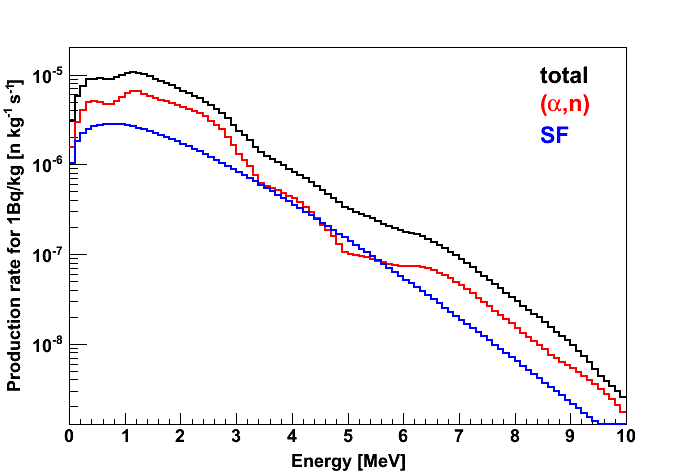
\includegraphics[width=0.475\linewidth]{plots/NRalphaN/NeutronProductionMaterials/steel-ProductionRate_for1Bq.png}
\label{figAlphaNproduction1Bq_1}}
\subfigure[PTFE]{
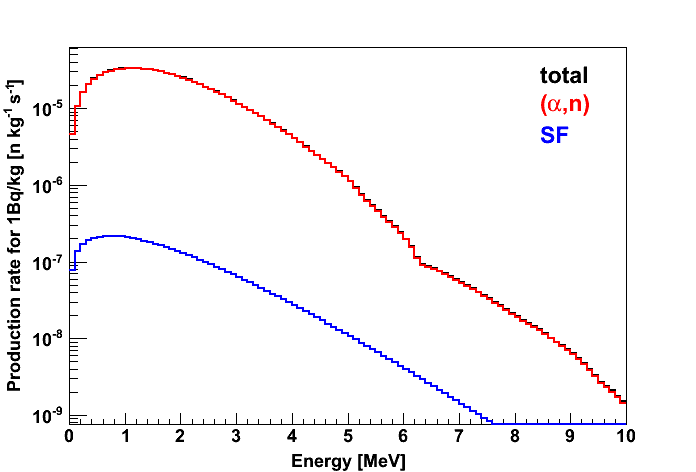
\includegraphics[width=0.475\linewidth]{plots/NRalphaN/NeutronProductionMaterials/teflon-ProductionRate_for1Bq.png}
\label{figAlphaNproduction1Bq_2}}
\subfigure[copper]{
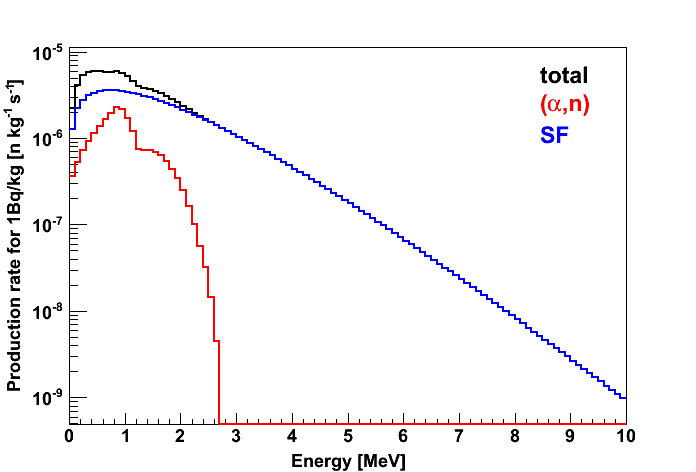
\includegraphics[width=0.475\linewidth]{plots/NRalphaN/NeutronProductionMaterials/copper-ProductionRate_for1Bq.png}
\label{figAlphaNproduction1Bq_3}}
\subfigure[lead]{
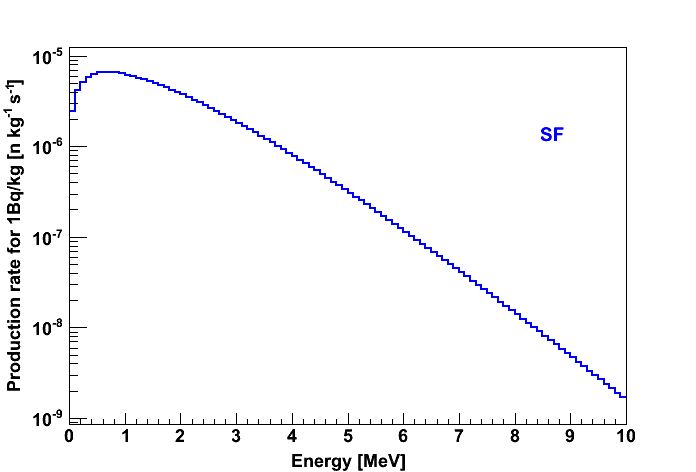
\includegraphics[width=0.475\linewidth]{plots/NRalphaN/NeutronProductionMaterials/lead-ProductionRate_for1Bq.png}
\label{figAlphaNproduction1Bq_4}}
\subfigure[PTFE]{
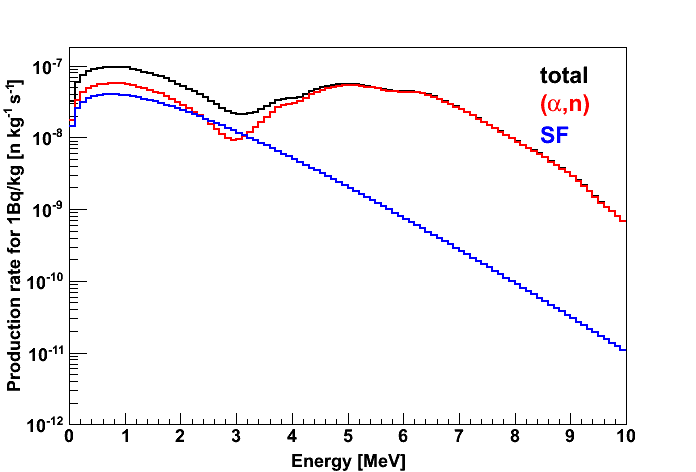
\includegraphics[width=0.475\linewidth]{plots/NRalphaN/NeutronProductionMaterials/poly-ProductionRate_for1Bq.png}
\label{figAlphaNproduction1Bq_5}}
\subfigure[ceramics]{
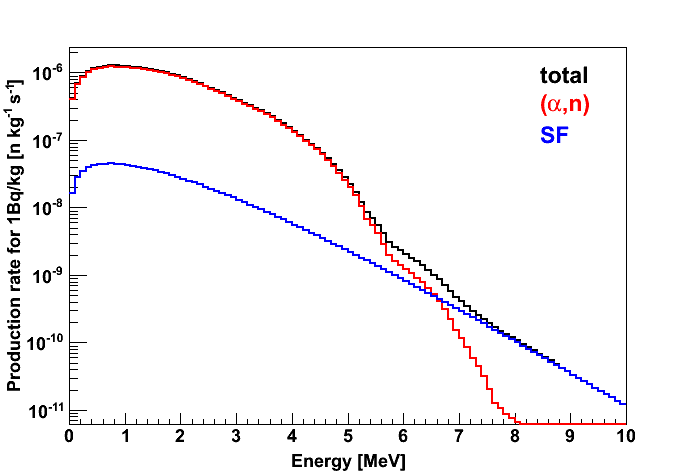
\includegraphics[width=0.475\linewidth]{plots/NRalphaN/NeutronProductionMaterials/ceramics-ProductionRate_for1Bq.png}
\label{figAlphaNproduction1Bq_6}}
\caption[Neutron production rates in ($\alpha$,n) and spontaneous fission reactions in materials of the XENON100 detector and its shield due to contamination of $^{238}$U, $^{235}$U and $^{232}$Th]{Neutron production rates in ($\alpha$,n) and spontaneous fission reactions in materials of the XENON100 detector and its shield due to contamination of $^{238}$U, $^{235}$U and $^{232}$Th. The neutron production is integrated in bins of 100~keV. Neutron production in light materials (with low atomic number $Z$), such as polyethylene, neutron the production rate is dominated by ($\alpha$,n) reactions. For high $Z$ materials, such as copper and lead, it is dominated by spontaneous fission reactions. The material with the highest neutron production is PTFE.}
\label{figAlphaNproduction1Bq}
\end{figure}

\begin{figure}[!b]
\centering
\subfigure[stainless steel]{
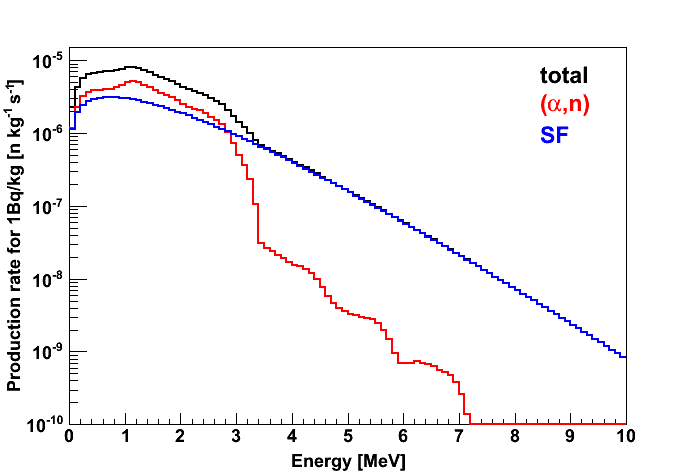
\includegraphics[width=0.475\linewidth]{plots/NRalphaN/NeutronProductionMaterials/pmt_metal1-ProductionRate_for1Bq.png}
\label{figAlphaNproduction1BqPMT_1}}
\subfigure[$Kovar$ metal]{
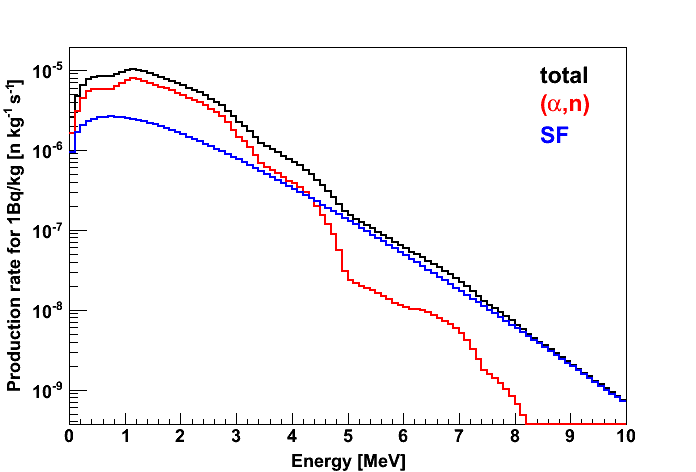
\includegraphics[width=0.475\linewidth]{plots/NRalphaN/NeutronProductionMaterials/pmt_metal2-ProductionRate_for1Bq.png}
\label{figAlphaNproduction1BqPMT_2}}
\subfigure[quartz]{
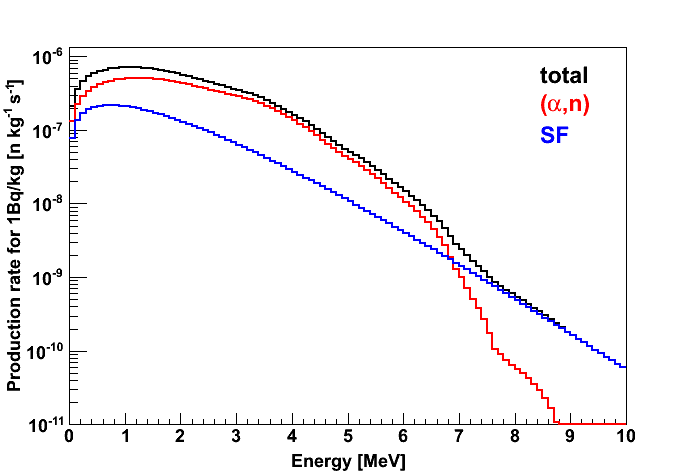
\includegraphics[width=0.475\linewidth]{plots/NRalphaN/NeutronProductionMaterials/pmt_quartz-ProductionRate_for1Bq.png}
\label{figAlphaNproduction1BqPMT_3}}
\subfigure[borosilicate glass]{
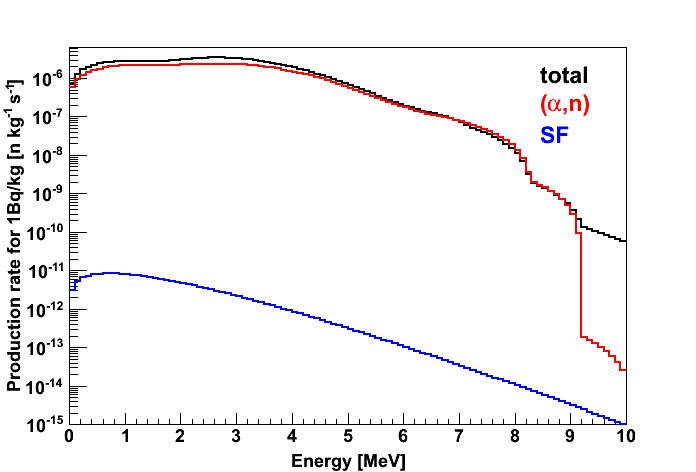
\includegraphics[width=0.475\linewidth]{plots/NRalphaN/NeutronProductionMaterials/pmt_glass-ProductionRate_for1Bq.png}
\label{figAlphaNproduction1BqPMT_4}}
\subfigure[aluminum]{
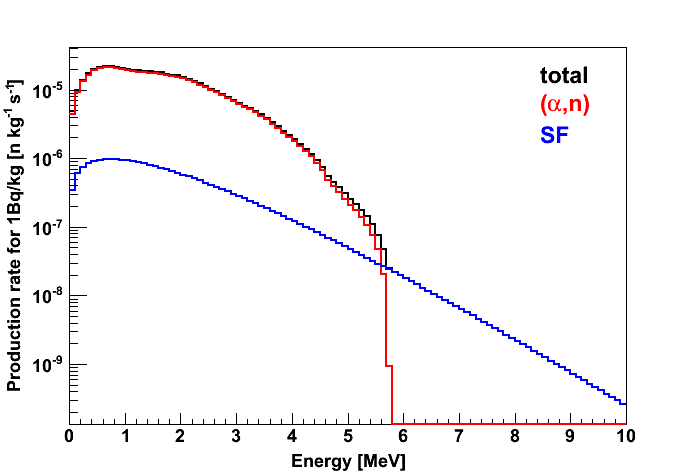
\includegraphics[width=0.475\linewidth]{plots/NRalphaN/NeutronProductionMaterials/pmt_Al-ProductionRate_for1Bq.png}
\label{figAlphaNproduction1BqPMT_5}}
\subfigure[$Cirlex$]{
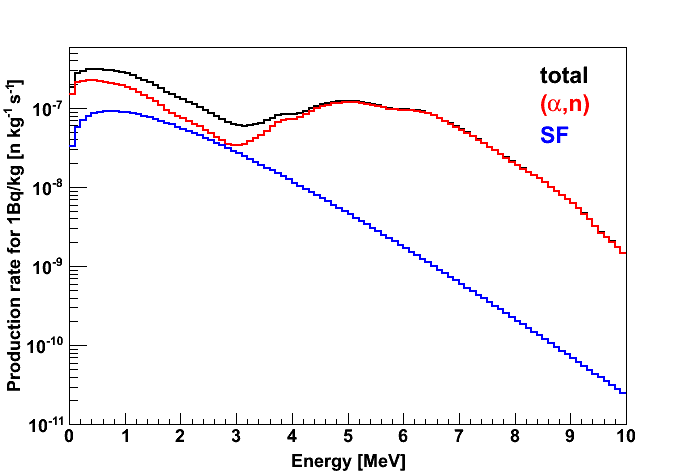
\includegraphics[width=0.475\linewidth]{plots/NRalphaN/NeutronProductionMaterials/cirlex-ProductionRate_for1Bq.png}
\label{figAlphaNproduction1BqPMT_6}}
\caption[Neutron production rates in ($\alpha$,n) and spontaneous fission reactions due to natural radioactivity in the materials of the PMTs and bases for the voltage divider network]{Neutron production rates in ($\alpha$,n) and spontaneous fission reactions due to natural radioactivity in the materials of the PMTs and bases for the voltage divider network. The stainless steel and $Kovar$ alloy dominate the neutron production in the PMTs.}
\label{figAlphaNproduction1BqPMT}
\end{figure}

The neutron production rates and their energy spectra have been calculated with the modified SOURCES-4A code~\cite{SourcesOriginal, SourcesModified}. The calculation has been performed for the case of $\alpha$-emitters distributed uniformly within the homogeneous  material. The program takes into account the energy-dependent ($\alpha$,n) cross sections and Q-values for all target nuclides, particle stopping cross sections for all elemental constituents, the energy of each $\alpha$-particle, and the spontaneous fission branching fractions for each source nuclide. As an input, the code requires the number of source and target nuclides, fractions of all atoms in each nuclide, the minimum and maximum neutron energy, and the number of neutron groups (bins). The fractions of atoms in the target material have been calculated using the chemical composition of the detector and shield material presented in Table~\ref{tabDetectorMaterials} and the natural isotopic abundance from Ref.~\cite{NuclearData}. The atom fraction of the parent isotope in a given material is calculated as:
\begin{equation}
f\ \text{[atoms/cm$^{3}$]} = \frac{N_{\mathrm{A}}}{A} \cdot \rho \cdot r \cdot q,
\end{equation}
where $N_{\mathrm{A}}$ - Avogadro constant [mol$^{-1}$], $A$ - atomic weight [g/mol], $\rho$ - material density [g/cm$^{3}$], $r$ - concentration of radioactive isotope [ppb mol/mol], $q$ - natural abundance of an isotope.

The calculation of atoms fractions of consequent $\alpha$-emitters takes into account the half-life time of the parent and daughter nuclei, assuming secular equilibrium within the decay chain.

The neutron production rate has been calculated for 1~kg of material and for contaminations of  $^{238}$U and $^{232}$Th of 1~Bq/kg. The secular equilibrium within $^{238}$U and $^{232}$Th decay chains has been assumed. The contamination of $^{235}$U has been calculated from the measured contamination of $^{238}$U, assuming the natural abundance of 0.72\%. The simulated neutron spectra are shown in Fig.~\ref{figAlphaNproduction1Bq}. The energy of the produced neutrons is limited to 10~MeV. The cross-section for the ($\alpha$,n) reaction decreases with the increase of the atomic number $Z$ of the target. This effect is  most pronounced for polyethylene, which consists of light elements (only carbon and hydrogen), hence the neutron production spectrum is dominated by ($\alpha$,n) reactions. In contrast, the neutron production in lead is entirely due to spontaneous fission reactions. 
The neutron spectra in the materials of the PMTs and bases for the voltage divider network are shown in Fig.~\ref{figAlphaNproduction1BqPMT}. The only low $Z$ material, for which the neutron production is dominated by ($\alpha$,n) reactions, is $Cirlex$.

The total neutron production from ($\alpha$,n) and spontaneous fission reactions has been calculated separately for the $^{238}$U (including the contribution from $^{235}$U) and $^{232}$Th chains, and is presented in Table~\ref{tabNeutronProductionMaterials}. Materials with the highest neutron production rates are PTFE, stainless steel, copper and lead. The PMT materials with the highest neutron production rates are aluminum, stainless steel and $Kovar$ alloy.

\begin{table}[!t]
\centering
\caption[Neutron production rate due to ($\alpha$,n) and spontaneous fission reactions in the XENON100 construction materials, calculated with SOURCES-4A]{Neutron production rate due to ($\alpha$,n) and spontaneous fission reactions in the XENON100 construction materials, calculated with SOURCES-4A. The systematic uncertainty of the code is $\pm$17\%.}
\label{tabNeutronProductionMaterials}
%\vspace{0.2cm}
\begin{tabular}{>{\footnotesize}l|>{\footnotesize}c|>{\footnotesize}c}
\hline
Materials 							& \multicolumn{2}{>{\footnotesize}c}{Neutron production [n$\cdot$kg$^{-1}\cdot$s$^{-1}$] for	1~Bq/kg of}	  \\
								&  $^{238}$U (incl. $^{235}$U) 			&  $^{232}$Th	  \\
\hline
316Ti stainless steel					&  (9.12$\pm$1.55)$\times$10$^{-5}$		& (1.43$\pm$0.24)$\times$10$^{-4}$ \\
PTFE							&  (3.27$\pm$0.56)$\times$10$^{-4}$		& (5.07$\pm$0.86)$\times$10$^{-4}$ \\
Copper							&  (8.93$\pm$1.52)$\times$10$^{-5}$		& (2.84$\pm$0.48)$\times$10$^{-5}$ \\
{\it Kovar} alloy						&  (8.97$\pm$1.53)$\times$10$^{-5}$		& (8.05$\pm$1.37)$\times$10$^{-5}$ \\
Stainless steel						&  (8.94$\pm$1.52)$\times$10$^{-5}$		& (1.35$\pm$0.23)$\times$10$^{-4}$ \\
Synthetic silica						&  (1.08$\pm$0.18)$\times$10$^{-5}$		& (1.01$\pm$0.17)$\times$10$^{-5}$ \\
Borosilicate glass					&  (5.53$\pm$0.94)$\times$10$^{-5}$		& (7.22$\pm$1.23)$\times$10$^{-5}$ \\
Aluminum 						&  (3.15$\pm$0.54)$\times$10$^{-4}$		& (6.03$\pm$1.03)$\times$10$^{-4}$ \\
Cirlex							&  (5.05$\pm$0.86)$\times$10$^{-6}$	 	& (4.94$\pm$0.84)$\times$10$^{-6}$ \\
Ceramics							&  (1.14$\pm$0.19)$\times$10$^{-5}$		& (1.98$\pm$0.34)$\times$10$^{-5}$ \\
Polyethylene						&  (2.11$\pm$0.36)$\times$10$^{-6}$		& (1.66$\pm$0.28)$\times$10$^{-6}$ \\
Lead								&  (1.56$\pm$0.27)$\times$10$^{-4}$		& (1.56$\pm$0.27)$\times$10$^{-4}$ \\
\hline
\end{tabular}
\end{table}

The total neutron production rate in the components of the XENON100 detector and its shield has been calculated by scaling the results of the calculation with SOURCES-4A to the mass of the materials, using the mass model introduced in Section~\ref{secGeant4model}, and the radioactive contamination measured with Ge detectors discussed in Section~\ref{secScreening}. The mass model of the R8520-06-Al PMT is described in Section~\ref{secPMT}. The results are presented in Table~\ref{tabTotalNeutronProductionComponents}.

The detector components with the highest neutron production rates are the lead and polyethylene shield layers, the detector cryostat and support bars made from 316Ti SS, PTFE and copper. The neutron production in the ceramics of the resistor chain for the field shaping rings is negligible due to its small mass. 
Even though the neutron production in aluminum of the PMTs is relatively high, it contributes little to the total neutron production in the PMTs due to the very low amount of material of only 0.1~g per PMT.

\begin{table}[!ht]
\centering
\caption[Neutron production rate due to ($\alpha$,n) and spontaneous fission reactions in the detector and shield components]{Neutron production rate due to ($\alpha$,n) and spontaneous fission reactions in the detector and shield components. The systematic uncertainty of the code is $\pm$17\%.}
\label{tabTotalNeutronProductionComponents}
%\vspace{0.2cm}
\begin{tabular}{>{\footnotesize}l|>{\footnotesize}c|>{\footnotesize}r|>{\footnotesize}r|>{\footnotesize}c}
\hline
Component  & Amount  & \multicolumn{2}{>{\footnotesize}c|}{Contamination [mBq]} & Neutron production \\
  		    & 		      & $^{238}$U & $^{232}$Th &  [neutrons/year] \\
\hline
Cryostat and `diving bell' (316Ti SS) 	& 73.61~kg 				& 1.65~/kg 		& 2.00~/kg 		& 14.53$\pm$2.47 \\
Support bars (316Ti SS)			& 49.68~kg 				& 1.30~/kg 		& 2.90~/kg 		& 12.36$\pm$2.10 \\
Detector PTFE 					& 11.86~kg 				& 0.06~/kg 		& 0.10~/kg 		& 5.42$\pm$0.92 \\
Detector copper 				& 3.88~kg 				& 0.16~/kg 		& 0.22~/kg 		& (3.72$\pm$0.63)$\times$10$^{-2}$ \\
PMTs 						& 242~pieces 				& 0.05~/pc		& 0.46~/pc		& 5.22$\pm$0.89 \\
PMT bases	 				& 242~pieces 				& 0.16~/pc		& 0.07~/pc		& 2.52$\pm$0.43 \\
TPC resistor chain 				& 1.5$\times$10$^{-3}$~kg 	& 0.014~/kg 		& 0.027~/kg 		& (2.72$\pm$0.46)$\times$10$^{-5}$ \\
Bottom electrodes (316Ti SS) 		& 0.23~kg 				& 1.90~/kg 		& 2.00~/kg 		& (4.63$\pm$0.79)$\times$10$^{-2}$ \\
Top electrodes (316Ti SS) 		& 0.24~kg 				& 3.60~/kg 		& 1.80~/kg 		& (5.91$\pm$1.01)$\times$10$^{-2}$ \\
PMT cables 					& 1.80~kg 				& 1.60~/kg 		& 3.70~/kg 		& (5.24$\pm$0.89)$\times$10$^{-2}$ \\
Copper shield					& 2.1$\times$10$^{3}$~kg 	& 0.083~/kg 		& 0.012~/kg 		& 6.32$\pm$1.07 \\
Polyethylene shield				& 1.6$\times$10$^{3}$~kg 	& 0.23~/kg 		& 0.094~/kg 		& 36.59$\pm$6.22 \\
Lead shield (inner layer)			& 6.6$\times$10$^{3}$~kg 	& 0.66~/kg 		& 0.55~/kg 		& 162.42$\pm$27.61 \\
Lead shield (outer layer)			& 27.2$\times$10$^{3}$~kg 	& 4.20~/kg 		& 0.52~/kg 		& (4.28$\pm$0.73)$\times$10$^{3}$ \\
\hline
\end{tabular}
\end{table}


